\chapter{Methods}
\label{chapter4}

When human's make decisions, they are often driven by previous experiences and some form of internal model of the world that we maintain. However, sometimes we question ourselves and think "what if this decision is better?"; this leads to us making different decisions, which are driven by reasoning. As an example, consider the route that you travel to work everyday. At some point you might question yourself and think "what if there is a faster route?", which may lead to you taking a longer route, by distance, because you think that there is a possibility that it could be faster. It might turn out that the longer route is indeed slower, and you may never try it again. However, it might be that you realise that the longer route is much faster, due to lack of congestion for example, and thereafter you follow it. This is the decision-making and reasoning process that we try to emulate.
\\Therefore, we propose a framework that synthesises planning and reinforcement learning which can overcome the inherent inaccuracies of models whilst constraining exploration  and improving sample efficiency by hypothesising, through reasoning, changes to the model that would be most beneficial to the planner and then planning on this temporary model to guide exploration. The correctness of these changes is then realised through experience in the real environment, and the model is updated.
We use the principle of \textit{optimism in the face of uncertainty}, we state that we are always almost in a state of uncertainty due to the inevitable inaccuracies of the model.
To enable the planner to make these hypotheses we equip it with additional actions which we denote Meta Actions.
\section{Meta Actions}
These actions do not cause the agent to act in the environment, and thus do not return any observation in terms of a new state and a reward, but rather cause changes directly to the model when called upon. An important factor and one of the main difficulties is deciding what Meta Actions should be exposed to the planner and when the planner should be able to invoke the Meta Actions. Therefore, we state three conditions which all must hold for a Meta Action to be invoked: a Meta Action must be admissible, feasible and reasonable.
\\A Meta Action is admissible if applying it to the model leads to what seems like a better plan: it must be optimistic. If applying the Meta Action does not result in any benefit to the planner, but rather it negatively affects the planner, then it should not be called. In-fact due to the nature of planning, an inadmissible Meta Action would never be called.\\Feasibility is important, since it ensures that we don't contradict observations and don't infinitely hypothesise changes to the model. However, the definition of feasibility depends on the transition dynamics of the domain. In the deterministic case, a Meta Action is feasible if the state or state-action pair that it affects has not been previously observed, and changes to to that state or state-action pair have not been previously hypothesised.
For stochastic domains, the latter condition of deterministic domains is sufficient for a Meta Action to be feasible.
\\Often, the change to the model that would be of most benefit the planner, is to simply add a transition from the current state to the goal state. However, this is almost never going to be a change that is realised to be correct; and instead would lead to behaviour akin to taking a random-walk through the state space until the goal is reached and the Meta Actions have been exhausted. Hence, it's key that an additional constraint exists, that ensures Meta Actions which are called hypothesise reasonable changes to the model. We consider two key ways of determining reasonability: through embedding reasonable Meta Actions in the model by-hand and through learning Meta Actions directly from experience.
\section{The Framework}
We assume that the environment has a discrete state space, $S$, or a state space that can be discretised, a finite action space, $A$, with deterministic or stochastic dynamics which can be described by a transition function, $T$, and deterministic rewards which can be described by a reward function, $R$. Therefore, we assume that the environment can be modelled as an MDP $E = (S, A, T, R)$, within which the agent acts at discrete time steps. The goal of the framework is to produce a policy, $\pi*$ which maximises the cumulative reward received when acting in the environment $E$.
Additionally, we assume that an attempt at modelling the environment has been made and embedded in an MDP $M = (S, A, T', R')$, where the same conditions hold for $T'$ and $R'$ as for $T$ and $R$. We do not expect or require $M$ to be accurate. 
\\We perform model-learning by maintaining $T'$ as a tabular maximum-likelihood model, and keep track of observed transitions using a function $n$ which maps state-action-state triples to an integer indicating how many times that transition has been observed.
\\We learn a tabular Quality Function, $Q$, through Q-Learning, which the policy $\pi$ is derived from. Q-Learning was chosen over SARSA, since it allows the optimal policy to be learnt independently of the current policy being followed; this suited our framework well, since we acknowledge that the policies followed during the exploration may not be optimal.
% The choice of initialisation open.
\\Our framework consists of two distinct phases: a planning phase where exploration takes place and a model-free phase. Since we only consider episodic tasks, the agent is given a finite number of episodes, $N_p$, for the planning phase, thereafter until termination (some finite number of episodes has been completed), the model-free learning takes over and the idea is that given sufficient model-free episodes $Q$ can converge to $Q^*$, and thus $\pi^*$ can be derived. Algorithm \ref{alg:framework_pc} gives a relatively high-level overview of the framework.

\begin{algorithm}
\caption{High-level Framework Pseudocode}
\label{alg:framework_pc}
\begin{algorithmic}
\REQUIRE $N$, number of episodes
\REQUIRE $N_p$, number of planning episodes
\REQUIRE $M$, model
\REQUIRE $s_s$, $s_g$, start, goal state
\ENSURE $\pi$, final policy
\STATE $i \leftarrow 0$
\STATE $Q(s,a) \leftarrow 0 $, $\forall s \in S$, $\forall a \in A$
\STATE $s \leftarrow s_s$
\FOR{$i=0$ to $N$}
    \STATE $Planning \leftarrow (i < N_p)$
    \WHILE{$s \neq s_g$}
        \IF{$Planning$ is \TRUE}
            \STATE $a \leftarrow$ Plan($s$, $s_g$)
        \ELSE
            \STATE $a \leftarrow \argmax_a Q(s,a)$
        \ENDIF
        \STATE Take action $a$ in state $s$, observe reward $r$ and new state $s'$
        \STATE Learn $Q$ according to observation.
        \IF{$Planning$ is \TRUE}
            \STATE Learn $M$ according to observation.
        \ENDIF
        $s \leftarrow s'$
    \ENDWHILE
\ENDFOR
\STATE $\pi(s) \leftarrow \argmax_a Q(s,a), \forall s \in S, \forall a \in A$
\RETURN $\pi$
\end{algorithmic}
\end{algorithm}


% \\Our framework consists of two phases, a planning phase and a model-free phase. 
%  Since we only consider episodic tasks, the agent is given a finite number of episodes, $N_p$ for the planning phase. The planning phase performs exploration and computes initial estimates for the Q-Values, $Q$. The model-free phase bootstraps from the initial Q-Value estimates and carries out model-free learning, following the policy $\pi_Q$, refining the estimate and continually updating the Q-Values.
\subsection{The Planning Phase}
The planning phase has three distinct steps: planning, acting and learning, which can be seen in Figure \ref{fig:planning_phase}. The goal of the planning phase is to perform exploration, and provide a good estimate for $Q*$ which the model-free learning can bootstrap and derive a policy from.

\begin{figure}[h!]
    \centering
    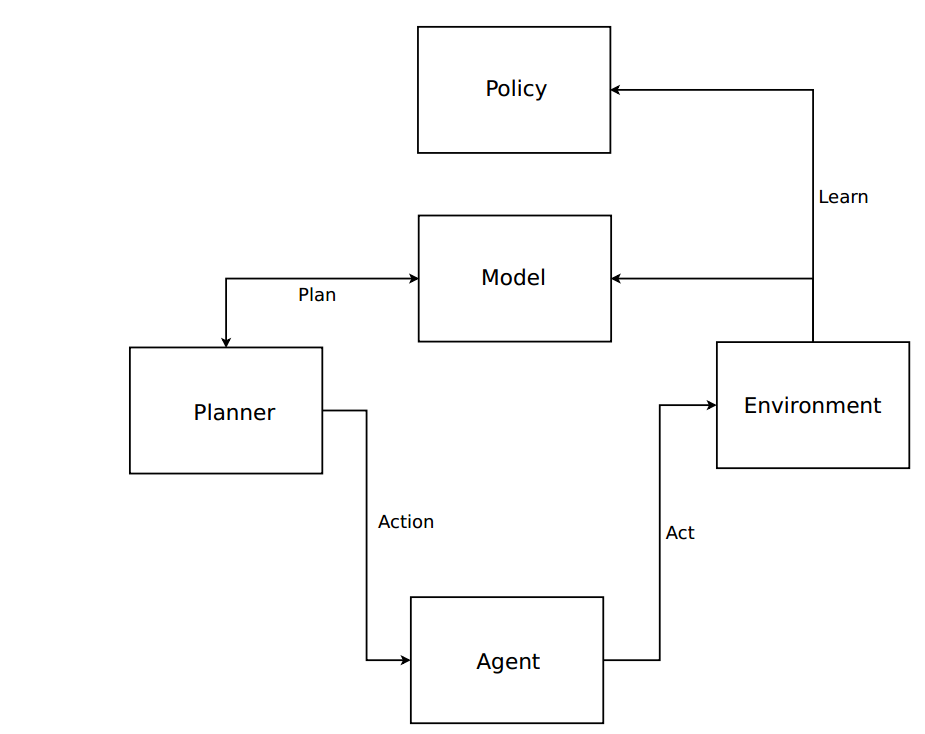
\includegraphics[max size={\textwidth}{\textheight}]{report/assets/planning_phase.png}
    \caption{Planning Phase}
    \label{fig:planning_phase}
\end{figure}

% Throughout the planing phase we maintain a tabular likelihood model which is used for model-learning, therefore we maintain a table $n$ which maps state-action-state triples to integers; for instance $(0, 1, 0) \rightarrow 3$ means that the transitions $(0, 1, 0)$ has been observed three times.
\subsubsection{Planning}
The planner constructs a temporary model, $M'$, which is identical to $M$. It then plans on $M'$ to produce a plan, $P$, from the current state $s$ to some goal, terminal, state $s_g$. The planner has access to the action space, $A$, as well as the additional Meta Actions. Whilst considering the Meta Actions, the planner may create additional temporary models, in order to evaluate the benefit of calling a particular Meta Action. If a Meta Action is chosen, then the temporary model $M'$ is updated, and planning continues. $P$ is maintained by the planner until $M$ is updated, when re-planning occurs. This ensures that unnecessary planning does not take place, saving on computational costs. However, this means that some mechanism needs to be in place for determining if the model has been altered since the last plan was generated; this can be a simple Boolean flag. $P$ is stored in a first-in, first-out (FIFO) data structure, such as a Queue. Thus, when the planner is invoked by the agent it simply removes and returns the top action.
\subsubsection{Acting}
At discrete time steps, $t$, the agent samples an action $a$ from the Planner, and executes it. At time $t+1$ it observes its new state $s'$ and the scalar reward signal.
\subsubsection{Learning}
The observation table is updated with the observed transition: $n(s, a, s') \leftarrow n(s, a, s')+1$, and if necessary the transition function, $T'$ of $M$ is updated by Equation \ref{eqn:tmlmupdate}. Furthermore, the reward function, $R'$, of $M$ is updated with the received reward, if necessary. $Q$ is updated according to the new state and reward received using Equation \ref{eqn:qlearningupdate}.
% We begin by updating the observation table $n$ with the observed transition. Then, we update the model, $M$ (if necessary). Furthermore, the $Q$-Function is updated according to the new state and reward received.
\subsection{The Model-Free Phase}
The model-free phase has two distinct steps: acting and learning, which can be seen in Figure \ref{fig:model_free_phase}. The goal of the model-free phase is to use pure model-free learning to bootstrap from the Q values learned during exploration, and get as close as possible to $Q^*$, so that $\pi^*$ can be derived.

\begin{figure}[h!]
    \centering
    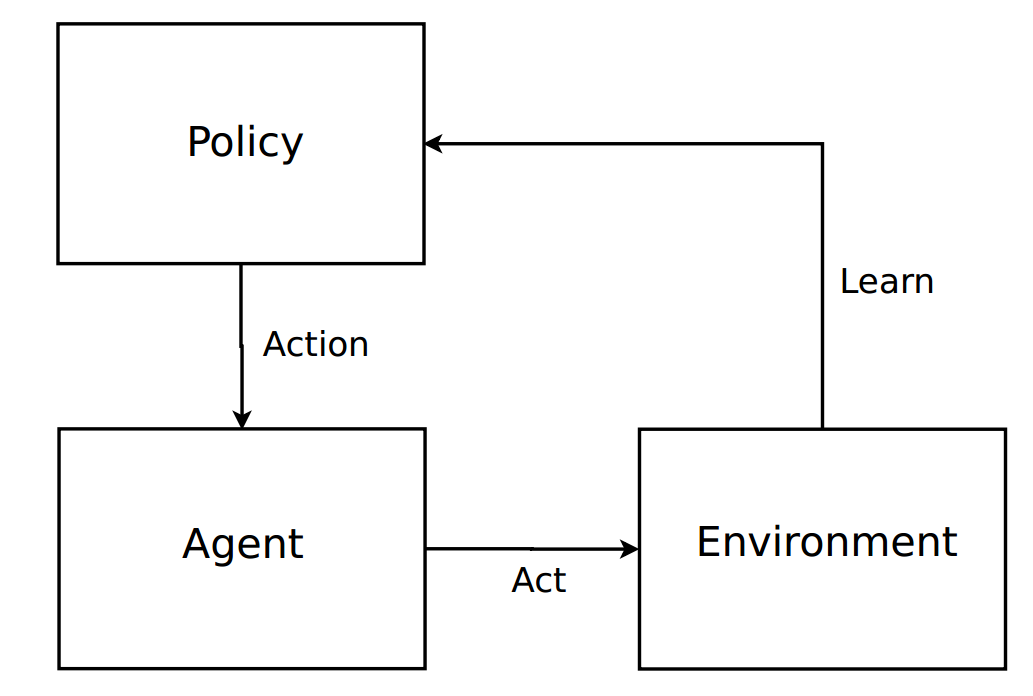
\includegraphics[max size={\textwidth}{\textheight}]{report/assets/model_free_phase.png}
    \caption{Model-Free Phase}
    \label{fig:model_free_phase}
\end{figure}

\subsubsection{Acting}
At discrete time steps, $t$, the agent greedily selections an action $a$ with respect to the $Q$, it selects the action according to the current policy, and executes it. At time $t+1$ it observes its new state $s'$ and the scalar reward signal.
\subsubsection{Learning}
$Q$ is updated according to the new state and reward received using Equation \ref{eqn:qlearningupdate}. Eventually, the updates will not result in changes to the policy, $\pi$, and therefore it will be continually followed until termination.
% \subsection{Planning}
% The choice of planner is largely irrelevant to the framework, we mostly consider heuristic search algorithms, through A*, and planning by dynamic programming, through Value Iteration. Value Iteration was chosen over Policy Iteration as it tends to be more efficient, and since we are performing VI many times; this is very beneficial. However, it is important for the planner to be able to quantitatively evaluate plans; planning by VI was a good option here, since it computed a Value Function as an intermediate step, and we could use that for evaluation.
% A temporary model is created. The planner then begins planning on this model, at each node (state), the planner considers both the actions and available Meta Actions - if a Meta Action is chosen, then that change is made to the temporary model and planning continues. The computed plan is then returned to the agent.
% \subsection{Execution}
% During the planning phase, the agent chooses actions by sampling a plan from the planner. During the model-free phase, the agent chooses actions from the learned policy. The agent then executes the action in the environment, observing its affects through its new state and the reward received.
% \subsection{Learning}
% There are two sections to the learning step: where the model is learned \citeppp{10.1145/122344.122377}, and  where the policy is learned. The model is learned, as a tabular maximum likelihood model. The policy is learned, by at each discrete time step  updating the maintained Q-values using Q-Learning.
% We acknowledge the fact that tabular maximum likelihood approach and tabular Q-function approaches do not scale well to large, continuous, state spaces, however the environments that we were interested in within this work had finite, discrete state spaces (or they could be discretised) which were not too large to suffer from the \textit{curse of dimensionality}. Moreover, these two choices allowed for simplifications to be made for ease of implementation. Q-Learning was chosen over SARSA, as it allows the optimal policy to be learned without actually following the optimal policy; this is key to the planning phase, where due to the hypotheses made, the policy being followed may not be optimal.
\section{Implementations}
The description of the framework above led to various implementations. The underlying concept of allowing the planner to hypothesise changes to the model through Meta Actions is present throughout all of the implementations. However, the choice of planning algorithm differs. Each implementation will be presented and highlighted here. Since in general the implementations follow the high-level overview provided in Algorithm \ref{alg:framework_pc}, we will not provide pseudocodes for each individual implementation, but we will however note where implementations differ.
\subsection{RL-A* Meta}
This was the initial implementation of the framework, and therefore the planner used was a simple heuristic search algorithm, A*; due to this choice, the implementation was limited to deterministic domains. This decision was made, as this implementation aimed at discovering if and when Meta Actions were useful. A* in particular was chosen due to ease of implementation. Furthermore A* maintains an evaluation function, $f$, which provided a good means of evaluating hypothetical changes made through Meta Actions.
\begin{equation}
\label{eqn:astareval}
f : S \times A \times S \rightarrow \mathbb{R}
\end{equation}
For the cost function,  it was intuitive to use the inverted reward function, namely $-R'$, this ensured that states with very negative reward were assigned a high cost and vice versa, leading to the following definition:
\begin{equation}
\label{eqn:astarevalsas}
f(s,a,s') = -R(s, a, s') + h(s')
\end{equation}
The choice of heuristic, $h$, relies on domain specific knowledge, therefore we do not define it here. However,  it remains that the heuristic must be admissible. The transition function was treated as a graph, which A* search was then performed on.
\\The Meta Actions that were available to the planner allowed it to add/remove transitions, and increase/decrease rewards for state-action-state triples, reasonable meta actions were embedded in the model by-hand. To ensure feasibility of Meta Actions and ensure that they were not infinitely called, a table was maintained which kept track of which Meta Actions had been called on which state-action-triples - this was used to ensure that each Meta Action can only be called once on each state-action-state triple. 
\subsection{RL-A* Meta with short-term memory}
This implementation was an extension of RL-A* Meta, which aimed to scale to stochastic domains. The stochastic nature means that the evaluation function once again needed to be modified, as such:
\begin{equation}
\label{eqn:astarevalsast}
f(s, a, s') = (1-T(s, a, s'))(-R(s,a, s')) + h(s')
\end{equation}
Since transitions were not guaranteed, the cost was weighted using the probability of the transition not occurring.
\\ The Meta Actions that were available to the planner allowed it to increase/decrease transition probabilities and increase/decrease rewards for state-action-state triples. Reasonable meta actions were embedded in the model by-hand. To ensure feasibility of Meta Actions and ensure that they were not infinitely called, a table was maintained which kept track of which Meta Actions had been called on which state-action-triples in the previous $N$ episodes, this is the short term memory.
\subsection{RL-VI Meta}
This implementations aims to deal with varying domains. We opted for planning by dynamic programming, namely through Value Iteration. Value Iteration was chosen because it allowed for us to easily evaluate plans (policies) through the Value Function. We chose Value Iteration over Policy Iteration, as Value Iteration is generally faster, and we needed to perform it many times.
\\The Meta Actions that were available to the planner allowed it to add/remove transitions, and increase/decrease rewards for state-action-state tuples, reasonable meta actions were embedded in the model by-hand. To ensure feasibility of Meta Actions and ensure that they were not infinitely called, a table was maintained which kept track of Meta Actions called within the current episode.
\subsection{RL-VI Meta, with learned Meta Actions}
The overall implementation is the same as RL-VI Meta, except Meta Actions are learned and obtained through experience, rather than embedded by-hand in the model. A Meta Action is learned when a discrepancy is noticed between the model and the real environment; this change that was applied to the model through model-learning becomes an action that can be invoked later on.